\section{Data sets}
\label{sec:observations}


\begin{figure*}
    \centering
    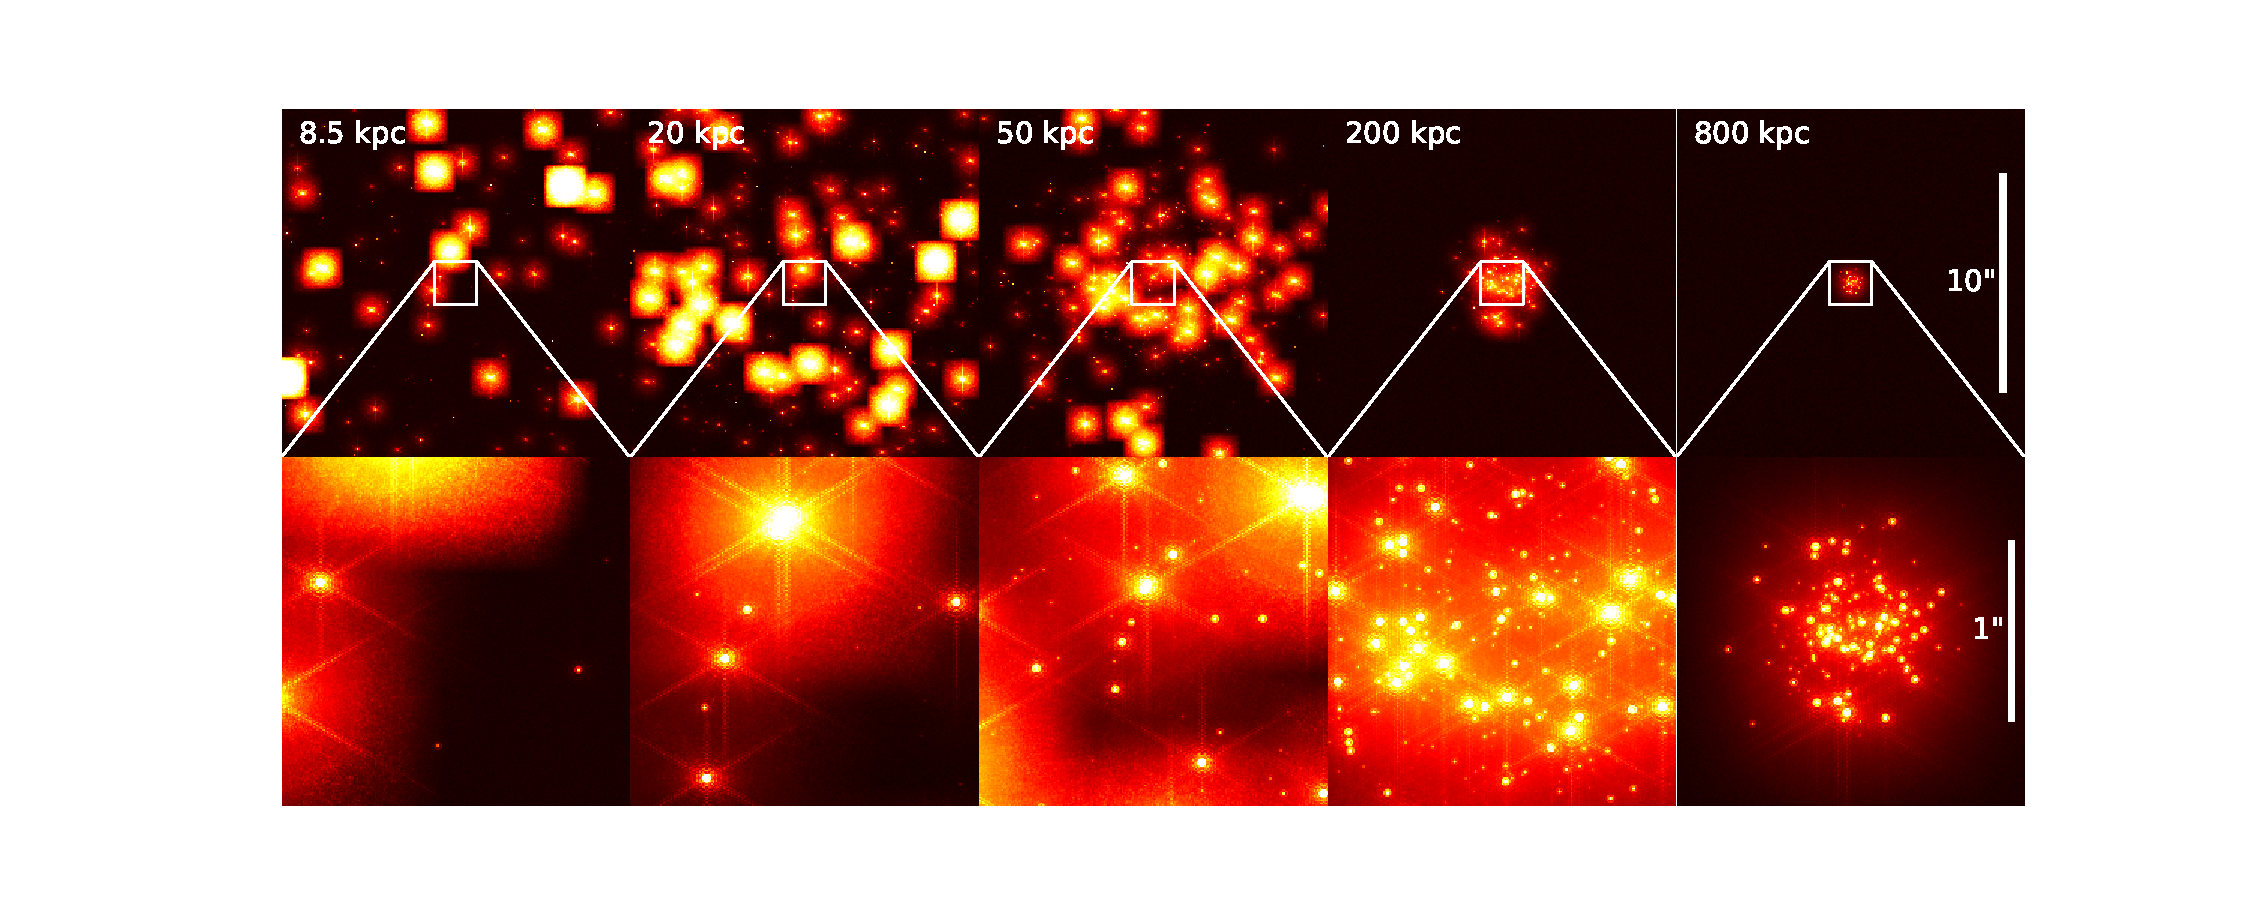
\includegraphics[width=\textwidth]{images/5_clusters.pdf}
    \caption{An illustration of the synthetic data used in this study. The model young massive cluster depicted here contains a mass of 2$\times$10$^4$\,\msun (approx. 5$\times$10$^4$ stars) and has a half-light radius of 1\,pc, and contains stars in the mass range [0.01, 100]\msun, sampled from a Kroupa IMF. The model cluster was observed with the MICADO instrument simulator (SimCADO) at distances from 8\,kpc to 800\,kpc. The top row shows the cluster as seen by the central detector of MICADO, (covering an on-sky area of 16\arcsec$\times$16\arcsec). The bottom row shows a 2\arcsec$\times$2\arcsec window (512$\times$512 pixels) at the center of this detector, corresponding to the area we used for our study. Here the unique structure of the ELT's PSF is visible. This Figure illustrates the difficulties that observers will face when studying crowded fields with MICADO and the ELT.
    }
    \label{fig:5_clusters}
\end{figure*}


\begin{figure*}
    \centering
    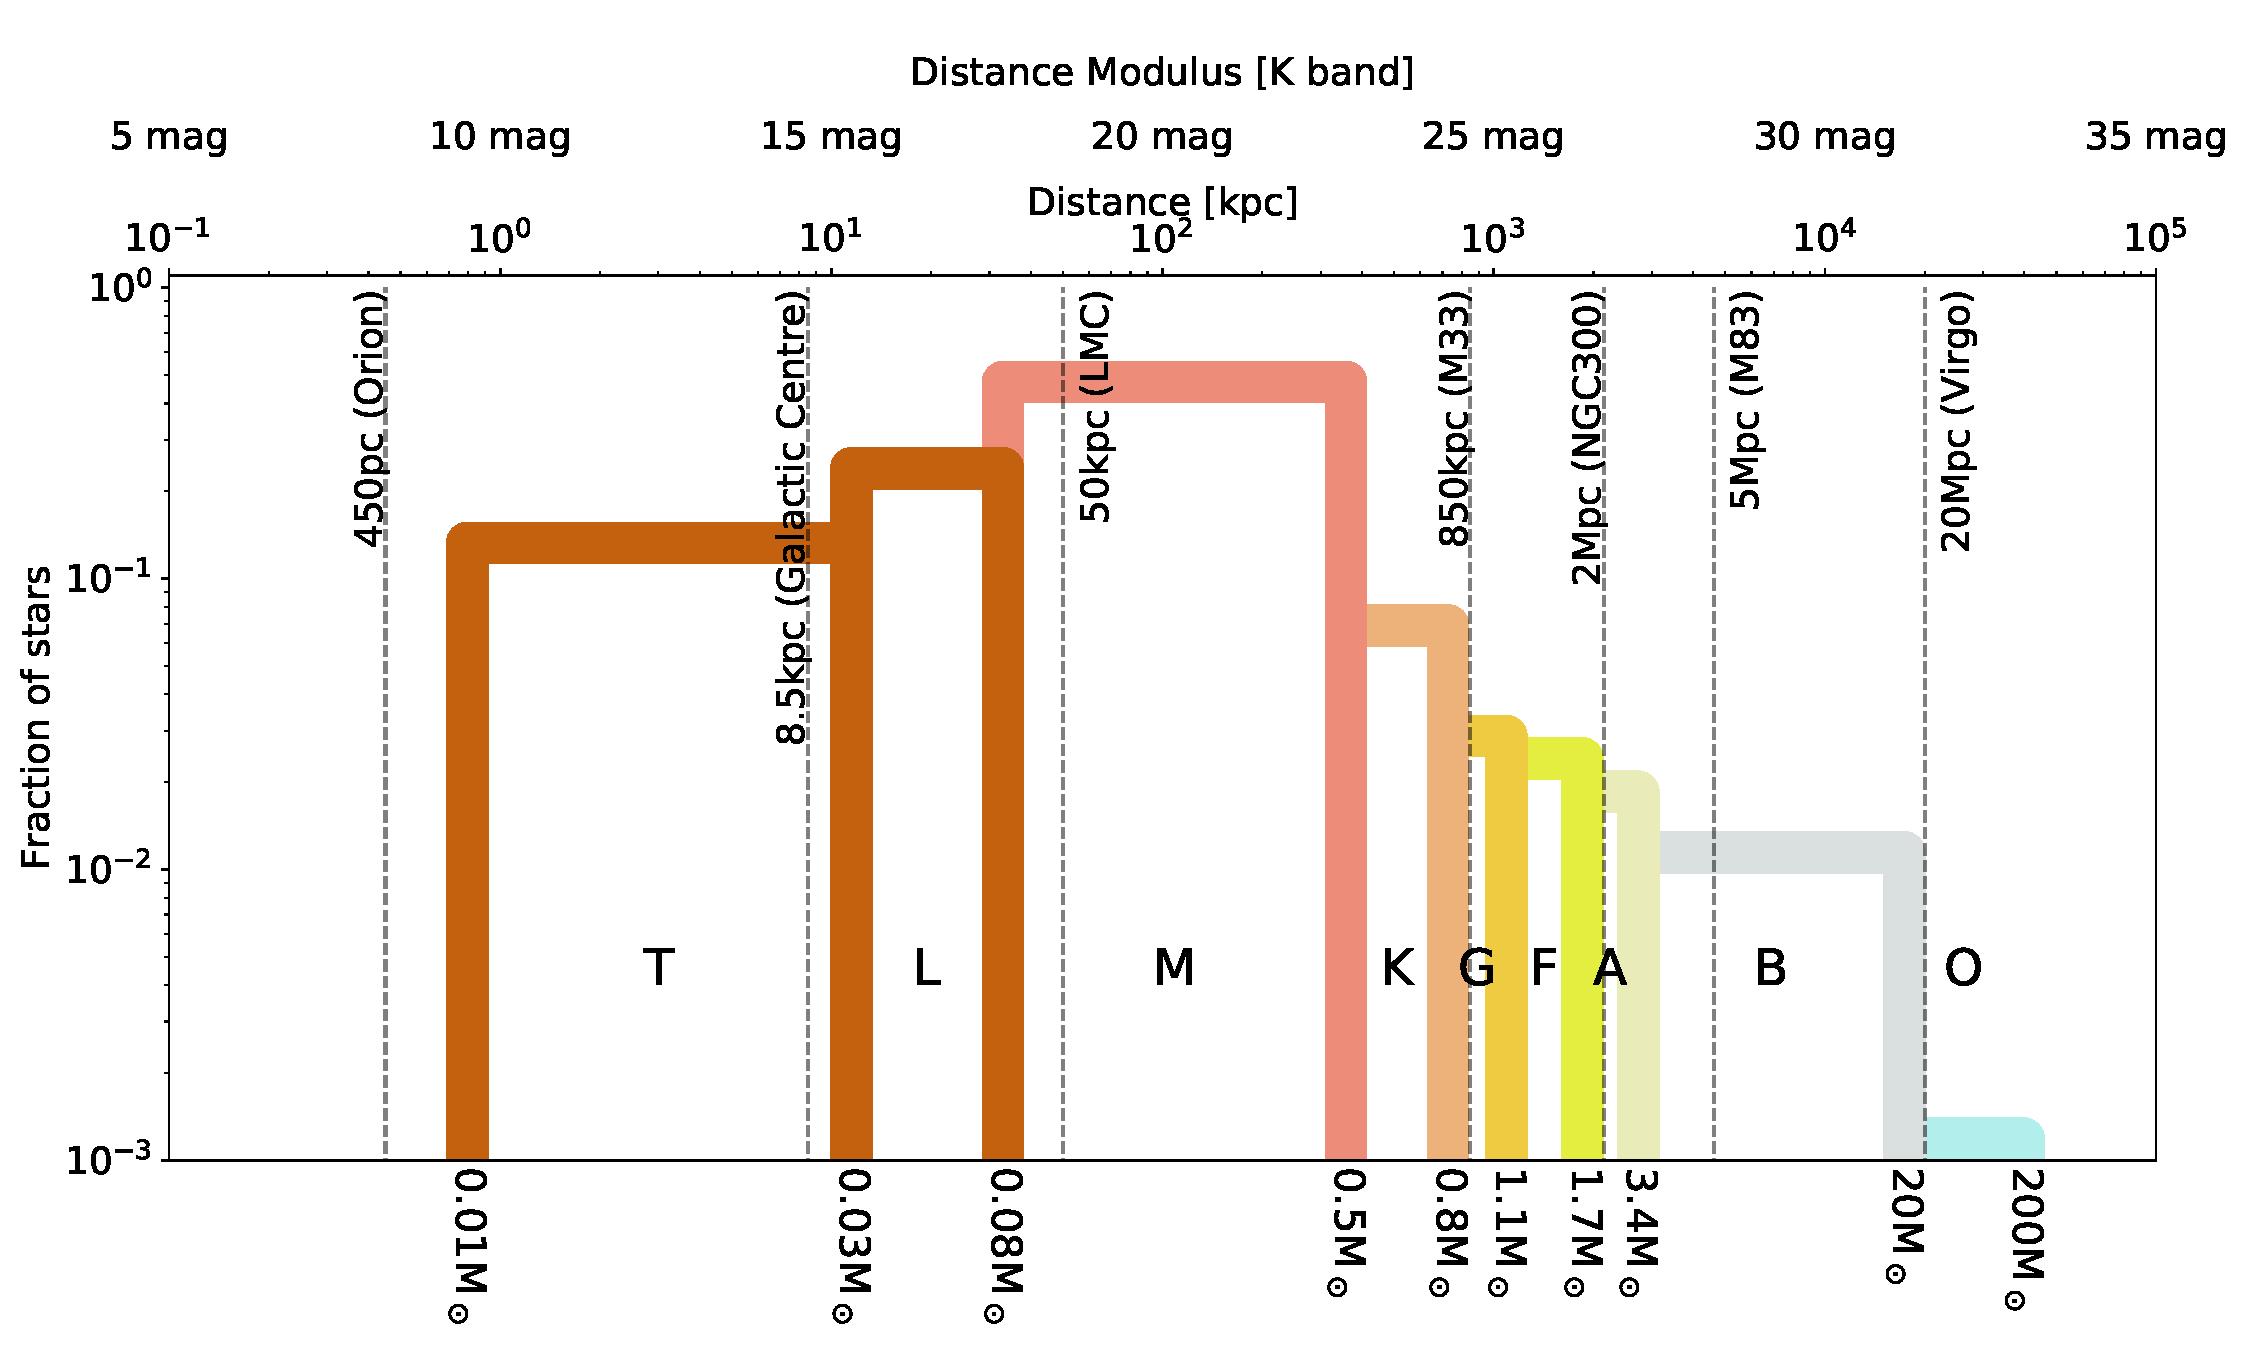
\includegraphics[width=\textwidth]{images/imf_educational.pdf}
    \caption{A qualitative illustration of the observational horizons of main sequence spectral types assuming a sensitivity limit of K$_S$=28$^m$ with MICADO and the ELT. The vertical dotted lines show the distance moduli of important regions for studying the IMF in environments significantly different to the solar neighbourhood. This height of each bar corresponds to the cumulative fraction of all stars belonging to a specific spectral type.
    }
    \label{fig:imf_educational}
\end{figure*}


\begin{figure*}

    \centering
    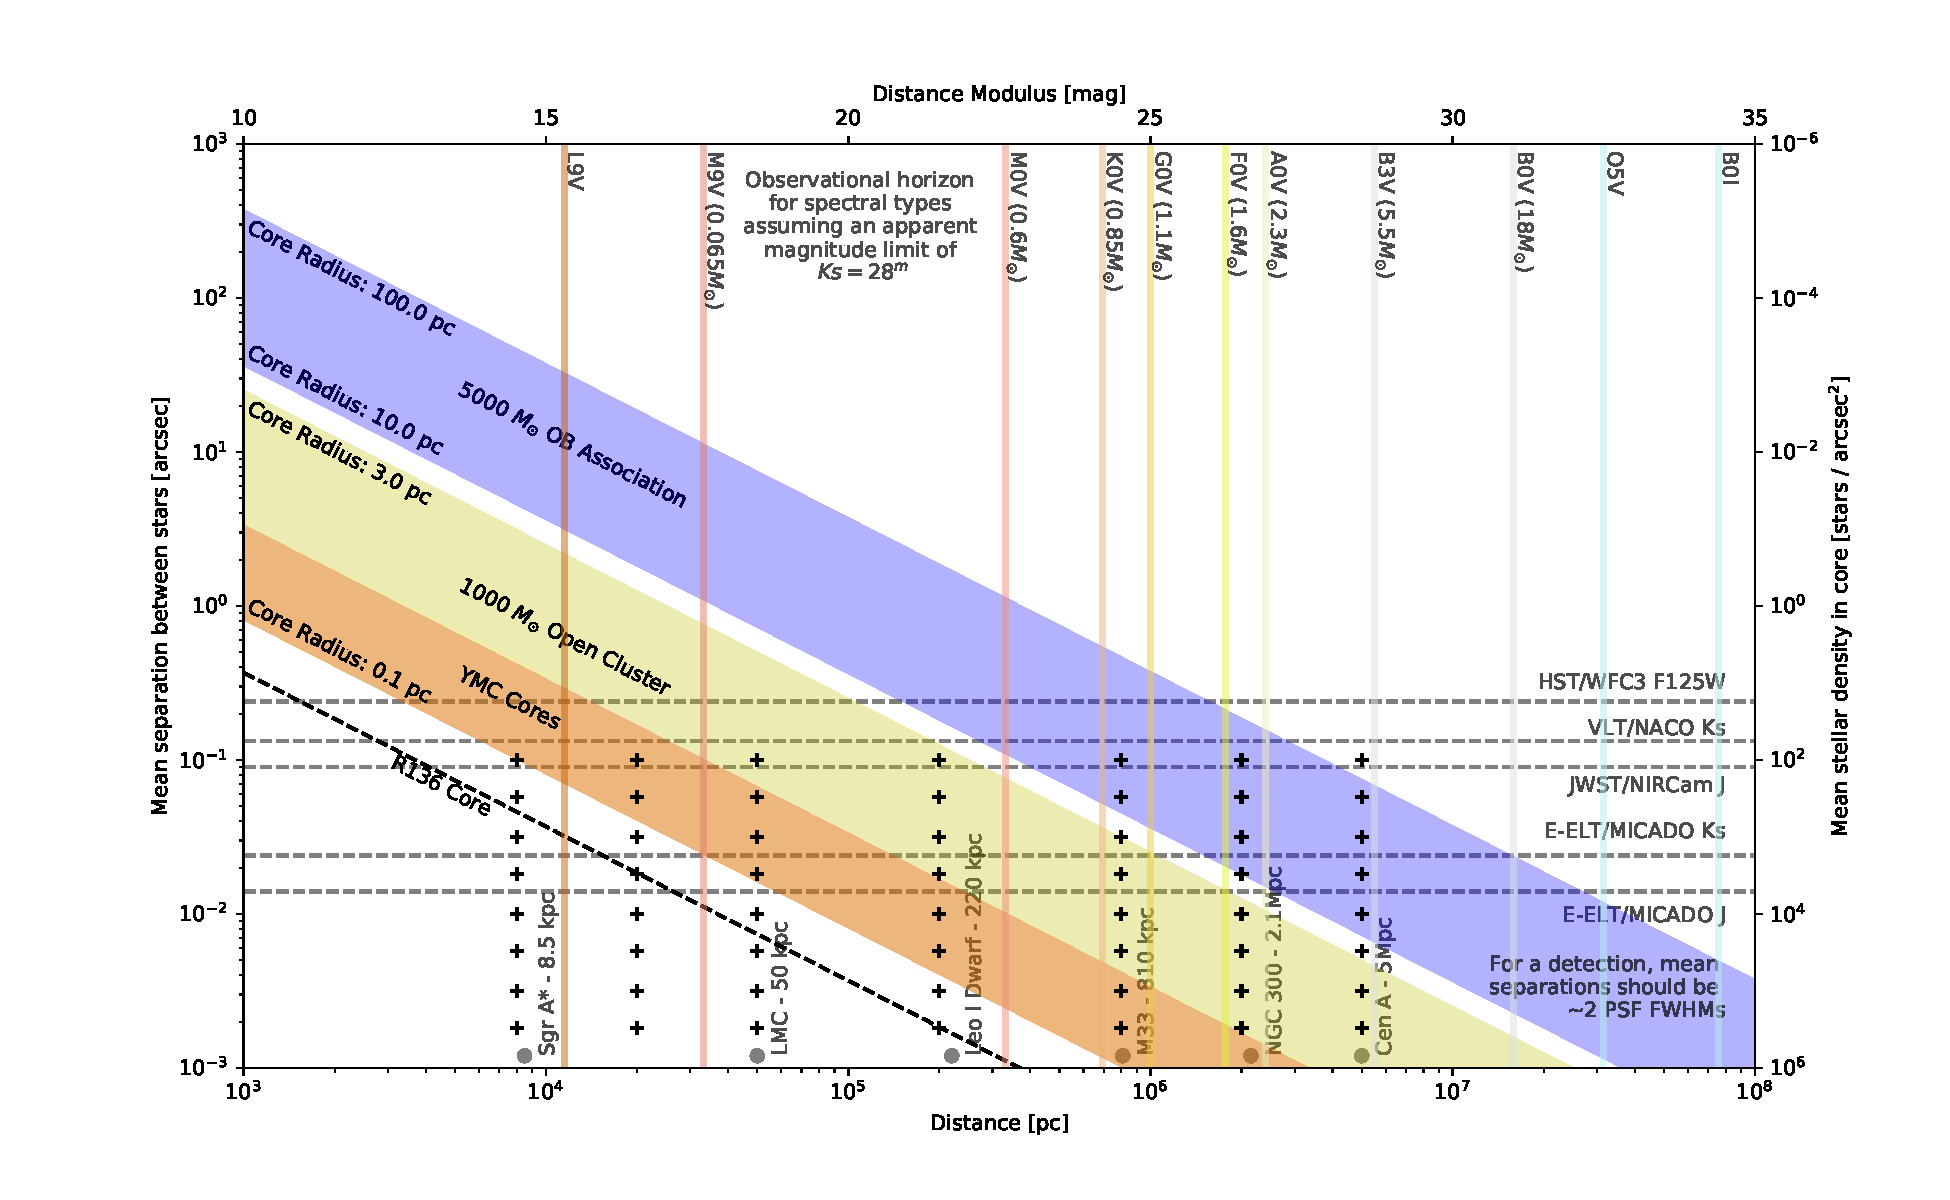
\includegraphics[width=\textwidth]{images/resolved_stellar_densities.pdf}

    \caption{Stellar density parameter space covered by the dense stellar fields in this study (crosses). 
    The diagonal bands represent the range of core densities for the three major categories of young stellar populations: young massive clusters (orange), open clusters (green), and OB associations (blue). 
    The vertical lines represent the furthest distance at which a particular type of main-sequence star will still be above the detection limit of MICADO, i.e., Ks=28\m. The dashed horizontal lines show the theoretical confusion limit for MICADO/ELT, JWST, HST, and an instrument similar to NACO/VLT. The confusion limit assumes an average minimum distance of 2$\times$ the PSF FWHM between stars.
    }
    
    \label{fig:resolved_stellar_densities}
    
\end{figure*}


The most reliable way to determine the IMF is to look at a population of stars that is still young enough for all (or most) of its original members to be around still, yet old enough that the main phase of star formation activity has ceased. 
If a population is too young, it will not have finished forming all its stars, and dust extinction will be a significant source of uncertainty and incompleteness. Too old and the most massive members will already have exploded as supernovae. 
Dynamical effects will also have lead to the evaporation of stars from the cluster, posing a problem to IMF completeness.
Unfortunately, such ideal conditions are rarely found. 
Star formation happens on time scales of 10\h6 years. 
The most massive stars burn their hydrogen reserves within the first few to several ten million years and move off the main sequence. 
Given that the dispersion time for stellar clusters is on the order of hundreds of millions of years (e.g., \citealt{Lada2003-ip}), at any point in time relatively few of the observable new clusters will be found in the ideal age range (between 5 and 20\,Myr) for studying the IMF. 
The majority of IMF studies focus on the clusters which come closest to meeting these conditions - namely the cores of open clusters (OC) and young massive clusters (YMC). 
OB associations also provide a laboratory for studying the IMF with the apparent advantage that stellar density does not pose a problem. However, as OB associations are spread out over distances as vast as a few hundred parsecs, the chances of contamination from background sources are higher. 
% Furthermore, the high mass end of the IMF cannot be reliably observed as the highest mass stars have already left the main sequence, and some have ended as supernova\correct.


\subsection{Parameter Space}

HST has a diffraction limit of \s0.1\arcsec at 1.2\,\um and can reach magnitudes as faint as J=28.6\m \citep{hst_wfc3} in a 10 hour observation. Using AO assisted ground-based instruments on 8\,m-class telescopes (similar to NACO at the VLT), diffraction-limited observations can be achieved over small (\s1\arcmin) fields of view. 
The diffraction limit of the VLT telescope (\s0.03\arcsec at 1.2\,\um) is \s3$\times$ smaller than HST, however, due to the atmospheric background, the sensitivity limits of VLT instruments are many magnitudes brighter than for HST. 
As boundary conditions for our suite of stellar fields, we took the resolution limit of HST, as cluster cores with densities lower than this are already accessible to the HST. 
Assuming an average of one star per FWHM of the PSF, our lower density limit was set to 100\,\spa. 
For the upper-density limit, we first took the theoretical diffraction limit of the ELT: 7\,mas at 1.2\,\ume, or 2$\times$10\h4\,\spae. 
As we wanted crowding-limited observations at large distances (\textgreater1\,Mpc), where the faint stars had already dropped below the sensitivity limit, we increased the true stellar density by a factor of 15$\times$ so that stars with masses M\,\textgreater\,1\,\msun alone would meet the crowding criterion of 1 star per FWHM. 
Thus we set the upper limit for the true cluster stellar density to 3$\times$10\h5\,\spa. 

Current telescopes are capable of detecting almost all main sequence stars above the hydrogen-burning limit (\s0.08\,\msune) within a few kiloparsecs of the Sun (e.g. \citealt{muzic17}). 
Detecting all main sequence stars in clusters further afield, e.g., in the galactic center and beyond, is where MICADO's increased sensitivity and resolution will bring the most significant breakthroughs. 
Indeed the question of whether the IMF is truly universal dictates that we study the IMF outside the Milky Way. 
Figure \ref{fig:imf_educational} illustrates the regions of the IMF that will be available to MICADO at various distances from Earth assuming a sensitivity limit of K$_S$=28$^m$. 
We therefore placed our model proxy-clusters at distances corresponding to important regions which will be critical for studying the effect of the interstellar environment on the IMF, e.g: The Galactic Centre (\s8\,kpc), the LMC (\s50\,kpc), Leo I dwarf galaxy (\s200\,kpc), M33 (\s850\,kpc)\footnote{We recognize that the location of the ELT in the southern hemisphere is unfavorable for effectively observing M33. We provide this data point because M33 will be observable by the Thirty Meter Telescope.}, NGC 300 (\s2\,Mpc), and M83 (\s5\,Mpc). 
Figure \ref{fig:resolved_stellar_densities} shows the parameter space covered by open clusters of average mass (\s1000\,\msun) with radii between 0.1\,pc and 3\,pc and OB Associations of average mass (\s5000\,\msun) with radii between 10\,pc and 100\,pc as distance from Earth increases. 
The lower bounds of the open cluster parameter space also cover the cores of YMCs. Average cluster properties were derived for the OB Associations from \citet{melnik1995}, for the open clusters from \citet{piskunov2007}, and for the YMCs from \citet{portegies2010}.


\subsection{Artificial stellar fields}
Figure \ref{fig:5_clusters} shows a model cluster placed at ever increasing distances from Earth. 
It is evident from Figure \ref{fig:5_clusters} that placing a single cluster at different distances would result in inhomogeneous datasets after running our source finding algorithm. 
In order to create a homogenous dataset that would allow for a direct comparison of the effects of distance and the ELT optics on crowded fields, we generated 56 densely populated stellar fields, that could function as proxies for the dense regions at the cores of young stellar clusters. 
Each stellar field was generated for a unique combination of stellar density and distance.
The parameter space covered by these cluster proxies is shown by the crosses in Figure \ref{fig:resolved_stellar_densities}. 
The size of each stellar field was set at 2\arcsec$\times$2\arcsec (see section \ref{sec:telescope}). 
The stellar fields were populated by continually drawing stars from an IMF until the required stellar density was reached. 
The mass of each star was drawn at random from an IMF distribution with minimum and maximum masses of 0.01\,\msun and 300\,\msun. 
The IMF followed a standard \citet{kroupa2001} broken power law distribution%with breaks at 0.08\,\msun and 0.5\,\msun and standard slope exponents
\footnote{By ``standard'' we mean: $\alpha=0.3$ for $\mathrm{M} < 0.08 \mathrm{M}_\odot$, $\alpha=1.3$ for $0.08\mathrm{M}_\odot < \mathrm{M} < 0.5 \mathrm{M}_\odot$, and $\alpha=2.3$ for $\mathrm{M} > 0.5 \mathrm{M}_\odot$ as defined in Kroupa (2001)}. 
Table~5 from \citet{pecaut2013}\footnote{Masses are not given in Table 5, but rather in the online supplement at \url{http://www.pas.rochester.edu/~emamajek/EEM_dwarf_UBVIJHK_colors_Teff.txt}}
was used to obtain the absolute J and Ks magnitudes for each star for the given mass. 
The requisite distance modulus for the stellar fields was added to give each star an apparent magnitude. 
We did not include extinction in the distance modulus, as this varies with the line of sight, in particular for Milky Way clusters. 
Since we are tackling the worst-case scenario, the core of the massive clusters, the stars were assigned random coordinates within the 2\arcsec$\times$2\arcsec bounding box. Real clusters will have a decreasing radial density profiles except for the inner cluster core radius, which will result in a easier characterization of the IMF over our conservative approach.

%\section{Simulations and data analysis}

\subsection{Observations}
\label{sec:telescope}

To ``observe'' our synthetic stellar fields we used the standard imaging mode of SimCADO\footnote{For documentation, see: \url{https://simcado.readthedocs.io/}. Github code base: \url{https://github.com/astronomyk/SimCADO}} \citep{leschinski2016}, an open-source instrument simulator which mimics observations with the wide-field mode of MICADO at the ELT. 
The core regions of open clusters and YMC have radii on the order of \s1\,pc \citep{portegies2010}. 
At a distance of 200\,kpc ($\sim$Leo 1 Dwarf), this translates to an angular diameter of \s2\arcsec. Thus we thought it safe to assume that the stellar density within the inner 2\arcsec$\times$2\arcsec region should remain relatively constant.
For the sake of computational effort, we decided to restrict to observations to this 2\arcsec$\times$2\arcsec window in the center of the detector.

At the very least dual-band photometry is required to determine the mass of a star. Therefore detections in at least the J and K$_S$ filters are necessary. 
We deemed a detection in the K$_S$ filter to be critical for any study of the IMF and therefore restricted our observations to this filter. 
The reason for this is as follows: The sky background in the K$_S$ filter is the highest of all NIR filters and the NIR stellar flux is for all main sequence stars (and many brown dwarfs) weakest in the K$_S$ filter. 
If a source is undetectable in the K$_S$ filter it will not be possible to determine its mass accurately. Given the AO-nature of the observations and the expected low Strehl ratio at 1.2\um \citep{clenet2016}, it could be argued that detections in the J filter will be more difficult. 
Ultimately the fluxes of the stars and the sky are set by nature, whereas the Strehl ratio is a question of engineering and optical design. 
The stars cannot be made brighter, whereas optical quality can be improved. 
Hence we deemed a detection in the K$_S$ filter to be the critical point for determining the mass of cluster members.
%This assumption comes with its own set of problems which will be discussed in a later paper.

Exposure times were kept to 1 hour for no other reason than observing time at the ELT will be in very high demand once it comes online, and observations in two or more filters are needed to accurately determine the mass of stars.


\subsection{Source extraction and matching}
Figures \ref{fig:results_lmc_1E3} and \ref{fig:results_lmc_1E4} in the Appendix show a graphical representation of the process described in this section. They show two examples of ``observed'' stellar fields placed at a distance of 50\,kpc and containing 10$^3$ and 10$^4$ \spa respectively. The stark features of the SCAO PSF
%\footnote{The PSF user here was from a simulation of the SCAO mode from MAORY. It was only released internally within the MAORY consortium. By default, the SimCADO package comes with a SCAO PSF generated by the MICADO consortium, which is in the public domain. \rewrite}
are clearly visible in the images. The diffraction core of the PSF is however still well modeled by a Gaussian distribution.
To find and measure the stars in the images we used the following method:

\begin{enumerate}
    \item Find the brightest star in the image with \verb+DAOStarFinder+ from \verb+photutils+ \citep{photutils}
    \item Find the center of the star in a 5$\times$5 pixel window around the coordinates given by \verb+DAOStarFinder+
    \item Fit a 2D Gaussian profile to the core of the star
    \item Scale an image of a reference star to match the amplitude, baseline and offset of the found star
    \item Subtract the scaled reference star from the image
    \item Repeat until \verb+DAOStarFinder+ no longer finds any sources above 5\,\sig
\end{enumerate}

In practice, we found that we could subtract \s100 stars at once and thus greatly increase the speed of the process. 
The amplitudes and baselines were converted to magnitudes based on the reference star. 
Our reference star was a solitary ``field'' star with a magnitude of K$_S$=15, observed for the minimum {MICADO} exposure time of 2.6\,s so as to maximize the signal-to-noise ratio while not saturating the detector. 
We calculated the mass of each star based on the observed fluxes in the K$_S$ filter. 
This step is only permissible because of the simplified context of this study. 
We were free to equate the luminosity function with an equivalent mass function because all our stellar fields have the intrinsic property that they only contain main sequence stars and the luminosity and mass functions enjoy a one-to-one relationship for this conversion in the K$_S$ filter, mathematically speaking. 
Furthermore, our primary goal is to determine what the lowest reliably observable mass is, based on how well MICADO will perform in crowded fields - not to directly measure the mass of the original stars. 
We are confident that this step does not significantly detract from achieving the goal of this study.

% We fitted the gaussian by flattening the star and the control star arrays, then doing linear regression to find the slope and intercept. We did this using scipy thielslope \textcolor{red}{wha??}

Finally, we cross-matched the coordinates of the extracted sources with the original table of coordinates to determine what fraction of stars were correctly detected with our algorithm. 
Due to noise and confusion from stars closer than a few FWHMs, the centroid coordinates of the extracted star were not always exactly equal to the original coordinates. 
The cross-matching algorithm was instructed to search for the closest star within a 25\,mas radius. 
If a fainter or brighter star happened to be closer, then the algorithm chose that star from the catalog as the match. 
We determined whether the extracted masses for stars in a certain mass bin were ``reliable'' by binning the extracted stars according to mass. We then took the mean and standard deviation of all stars within a mass bin. 
As long as the mean extracted mass to true mass ratio was in the range 1.0$\pm$0.1 and the standard deviation was less than 0.1, the mass bin was classed as reliable. By this definition, the lowest reliably detectable mass for a stellar field was given by the lower edge of the lowest mass bin which satisfied these criteria.

